\section{Empirical Evidence}

The empirical analysis has two purposes. Its primary purpose is to show that the
coding framework distinguishes official compliance from the institutional
location of local public-finance functions. Its secondary purpose is to examine
whether one historical indicator of local administrative development is
associated with the observed fates. The second exercise is exploratory. The
reference sample was not drawn to estimate national outcome frequencies, the
institutional-change outcome is sparse, and the available adjusted models are
sensitive to sample composition.

\subsection{Working reference labels and source traceability}

The working-reference file contains 94 city-platform cases assigned through
Codex source-packet review on behalf of the project author under the frozen
codebook. The author subsequently reported human checking of all 94 labels
without revision, as documented in the measurement audit. Each case records a formal event, the
post-event location of the relevant function, the final label, a plausible
alternative, and three evidence-quality scores. The labels comprise two
substantive exits, 82 nominal exits, ten functional transfers, and no
liquidations. This distribution demonstrates that the categories can be
applied to documentary evidence, but it is not a population estimate. Cases
were assembled to develop and stress-test the measure rather than sampled from
a national issuer frame.

Eighty-four reference cases match the CBDB-GADM historical crosswalk used in
the exploratory application. The ten unmatched cases remain in the measurement
file but not in the historical-capacity tables. Table
\ref{tab:pilot-validation-tiers} separates these analytical objects from the
larger disclosure-screening pool.

% Auto-generated by scripts/build_pilot_capacity_summary.py
\begin{table}[htbp]
\centering
\caption{Measurement files used in the empirical analysis}
\label{tab:pilot-validation-tiers}
\begin{tabular}{@{}lrl@{}}
\toprule
Tier & Cases & Use in the paper \\
\midrule
Author-reviewed reference file & 94 & Documentary outcome reference \\
Historically matched reference subset & 84 & Used for exploratory descriptive tables \\
Candidate disclosure pool & 361 & Used for LLM-assisted screening \\
Usable screening rows & 346 & Source-backed screening coverage \\
One-sided surrogate disclosure labels & 203 & Provisional nominal-exit screens \\
\bottomrule
\end{tabular}
\begin{minipage}{0.96\linewidth}
\vspace{0.5em}\footnotesize Notes: The reference labels were reviewed by the
project author and have not yet been independently double-coded. The
historically matched subset is smaller because the current CBDB-GADM crosswalk
does not contain usable matches for 10 reference cases. Candidate
disclosures and surrogate rows are source packets rather than final city-platform labels.
\end{minipage}
\end{table}


The source reconstruction audit establishes a different form of credibility.
All 94 evidence identifiers resolve to the source inventory, 93 cases have
complete local copies of every cited document, all 94 have recovery URLs for
their cited documents, and 62 have exact case-level evidence memos. Appendix
Table \ref{tab:pilot-source-audit} reports the formal event, post-event function,
source basis, and final label for the historically matched cases. Traceability
does not establish intercoder reliability, but it allows readers to reconstruct
the documentary judgment and to distinguish a missing source from a disputed
classification.

\subsection{Institutional variation}

Table \ref{tab:pilot-capacity-bin-exit-type} reports the observed labels across
three historical elite-density bins. The low bin contains only nominal exits.
The middle bin contains nominal exits and functional transfers. The high bin
contains all three observed fates, including both substantive exits. Nominal
exit nevertheless remains the modal outcome in every bin.

% Auto-generated by scripts/build_pilot_capacity_summary.py
\begin{table}[htbp]
\centering
\caption{Historical capacity bin and validated exit type}
\label{tab:pilot-capacity-bin-exit-type}
\begin{tabular}{@{}lrrrr@{}}
\toprule
Historical capacity bin & Substantive & Nominal & Functional transfer & Total \\
\midrule
High historical capacity & 2 & 19 & 5 & 26 \\
Middle historical capacity & 0 & 20 & 5 & 25 \\
Low historical capacity & 0 & 26 & 0 & 26 \\
\bottomrule
\end{tabular}
\begin{minipage}{0.92\linewidth}
\vspace{0.5em}\footnotesize Notes: The table uses only the 77 historically matched human-validated pilot labels. Capacity bins are assigned from the CBDB-GADM Ming-Qing elite-density measure among matched human-validated cases. Counts are descriptive and are not population estimates.
\end{minipage}
\end{table}


Figure \ref{fig:pilot-exit-type-by-capacity-bin} displays the same pattern as
within-bin shares. It serves the measurement argument more directly than a
ranking of historical elite density because it shows the institutional outcome
that official exit counts leave unobserved.

\begin{figure}[htbp]
\centering
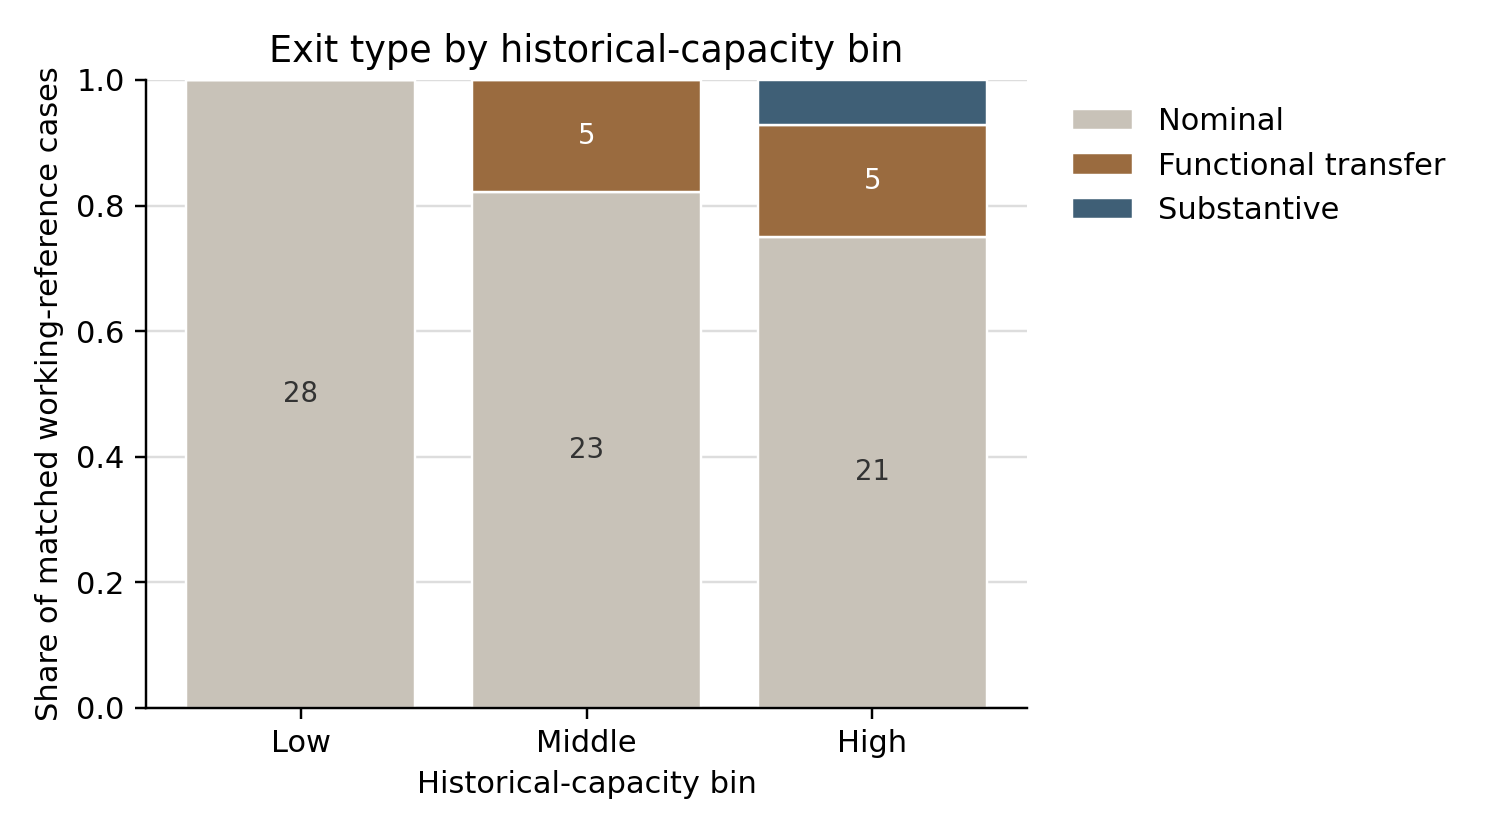
\includegraphics[width=0.82\linewidth]{figures/pilot_exit_type_by_capacity_bin.png}
\caption{Exit type by historical-capacity bin}
\label{fig:pilot-exit-type-by-capacity-bin}
\end{figure}

The case evidence clarifies the distinctions. Guangzhou City Construction
Investment and Ningbo Development Investment receive substantive-exit labels
because the reviewed packets indicate movement away from off-budget
government-project financing. Guangzhou's former government project work is
described as fiscally funded entrusted management rather than financing by the
platform. Xuzhou, Yancheng, and Hengyang receive nominal-exit labels because
formal exit or no-government-financing language coexists with infrastructure
construction, land preparation, government settlement, fiscal support,
repayment exposure, or entrusted construction. Hangzhou and Wenzhou illustrate
functional transfer: the public function remains in a reorganized municipal
state-owned system even though its issuer or organizational location changes.

These contrasts do not imply that historical capacity determines fate. The
reference set contains many high-capacity nominal exits. They show that strong
administrative inheritance can coexist with continuing platform finance when
development-zone mandates, debt pressure, land dependence, or local investment
commitments preserve the demand for an off-budget organization.

\subsection{Exploratory historical association}

The statistical application defines institutional change as substantive exit or
functional transfer, with nominal exit as zero. This binary outcome does not
collapse the conceptual distinction between absorption and transfer. It
provides a feasible exploratory comparison because the matched sample contains
only two substantive exits and no liquidation.

% Publication-facing rendering of EXP-20260830-012.
\begin{table}[htbp]
\centering
\caption{Exploratory sparse-outcome audit of historical capacity}
\label{tab:exploratory-sparse-outcome-audit}
\small
\setlength{\tabcolsep}{4pt}
\begin{tabular}{@{}lcccc@{}}
\toprule
 & Hist. LPM & Hist. Firth & Adj. LPM & Adj. Firth \\
\midrule
Elite-density effect & 0.066 & 0.056 & 0.005 & 0.003 \\
 & (0.041) & (0.032) & (0.045) & (0.052) \\
\midrule
Observations & 84 & 84 & 78 & 78 \\
Institutional-change events & 12 & 12 & 12 & 12 \\
Contemporary controls & No & No & Yes & Yes \\
Province fixed effects & No & No & No & No \\
\bottomrule
\end{tabular}
\begin{minipage}{0.94\linewidth}
\vspace{0.5em}\footnotesize Notes: This table is an exploratory diagnostic, not
a causal estimate. The outcome equals one for substantive exit or functional
transfer and zero for nominal exit. Effects are probability-point changes for
a one-sample-standard-deviation increase in elite density. LPM uncertainty is
HC1. Firth effects are average marginal effects with curvature-based
delta-method uncertainty shown only as a diagnostic. Adjusted models use
district-and-county platforms as the reference category. All fixed models were
reported without selection by sign or statistical significance.
\end{minipage}
\end{table}


Table~\ref{tab:exploratory-sparse-outcome-audit} reports the full fixed set of
historical-only and adjusted specifications. In the 84 matched cases, a
one-standard-deviation increase in historical elite density is associated with
a 6.6 percentage point increase in institutional change in the linear
probability model and a 5.6 percentage point average marginal effect in the
Firth logit. Their respective 95 percent diagnostic intervals are
$[-1.3,14.6]$ and $[-0.8,11.9]$ percentage points; both include zero.
Appendix Table~\ref{tab:pilot-lpm-institutional-change} retains the alternative
high-capacity and ordered-bin comparisons. The estimates describe the
assembled cases rather than a national probability sample. Elite density may
also capture persistent education or social capital.

The adjusted results are less stable. Contemporary controls are available for
78 of the 84 matched cases. Complete-case restriction removes six low-capacity
nominal exits while retaining all twelve institutional-change events. A
preregistered audit repairs the former rank deficiency by using
district-and-county platforms as the reference category. The corrected design
has eight independent columns and twelve events, or 1.5 events per column. The
adjusted linear probability and Firth-logit effects are 0.5 and 0.3 percentage
points. Deleting one observation at a time changes their signs in nine and
eleven of 78 fits, respectively. The two historical-only effects change sign
in zero deletions. Province fixed effects are not estimated because
only four of eighteen provinces have within-province outcome variation and the
candidate design would contain 25 columns for twelve events. Contemporary
fiscal capacity, debt pressure, land-finance dependence,
province, disclosure quality, platform level, and capital or sub-provincial
status remain alternative explanations rather than established controls for a
causal historical effect.

\subsection{LLM screening and the validation boundary}

The LLM-assisted file expands documentary screening without expanding the set
of final outcomes. Among 361 candidate disclosure rows, 346 have usable source
text or a reviewed status. The exit-type portion contains the 94 reference
labels and 203 one-sided nominal-exit surrogates. Forty-four reviewed packets
lack a directly documented formal event, five are boundary packets, and fifteen
lack a usable source packet.

% Auto-generated by scripts/build_llm_screening_sample.py
\begin{table}[htbp]
\centering
\caption{LLM screening status for the candidate pool}
\label{tab:llm-screening-status}
\small
\begin{tabular}{@{}lrr@{}}
\toprule
Screening status & Rows & Use \\
\midrule
Working reference label & 94 & Provisional documentary outcome \\
LLM surrogate exit type & 203 & One-sided provisional nominal screen \\
LLM screened, no direct formal event & 44 & Screened non-outcome \\
Source-packet-reviewed boundary & 5 & Scope condition \\
Source packet missing & 15 & Not usable \\
\midrule
Usable LLM screening rows & 346 & Screening sample \\
Usable exit-type rows & 297 & Outcome sample \\
\bottomrule
\end{tabular}
\begin{minipage}{0.94\linewidth}
\vspace{0.5em}\footnotesize Notes: A usable screening row has a working reference label, an LLM surrogate label, a source-packet-reviewed boundary decision, or source text screened as lacking a direct formal event. Working reference labels await independent human confirmation. Surrogate rows are not final four-category outcomes. Rows without a codable formal event are not assigned substantive, nominal, functional-transfer, or liquidation labels.
\end{minipage}
\end{table}


Repeated disclosures reduce the 203 surrogate rows to 158 issuers. Sixty-one
issuers also appear in the reference file; 97 do not. The 61 overlapping
issuers receive nominal labels under both procedures. This exact agreement
shows that the narrow screen can recover a documentary pattern already
recognized by the codebook. It is not probability-sample precision. The
overlap was formed after positive screening, and no screen-negative issuer has
a working-reference label. The data therefore do not identify recall,
four-category calibration, or error among screen-negative cases.

Table~\ref{tab:validation-identification-bounds} quantifies what the missing
labels permit without assuming that the observed overlap represents the other
issuers. If $K_+$ reference outcomes establish membership in a class, $K_-$
establish nonmembership, and $U$ are unknown, the finite-screen share lies
between $K_+/N$ and $(K_++U)/N$. For the 158 screen-positive issuers, the
conditional bounds are 38.61 to 100 percent. This wide range is compatible
with the selected 61-of-61 concordance because 97 issuer outcomes remain
unknown.

These bounds require the linked reference labels to be correct and applicable
to the corresponding issuer and event. Shared source documents are found for
41 links, but issuer matching and documentary overlap do not establish
independent same-event pairing. Without the applicability assumption, the
unconditional bounds are zero to 100 percent. The table therefore reports
identified sets conditional on stated evidence, not accuracy confidence
intervals, and it does not turn excluded or no-event cases into negative
outcomes.

% Generated by scripts/build_validation_identification_bounds.py; EXP-20260910-006
\begin{table}[htbp]
\centering
\small
\caption{Conditional finite-screen identification bounds}
\label{tab:validation-identification-bounds}
\setlength{\tabcolsep}{3pt}
\begin{tabular}{@{}lrrrrrr@{}}
\toprule
Population and quantity & $N$ & $K_+$ & $K_-$ & $U$ & Lower & Upper \\
\midrule
Screen: nominal membership & 158 & 61 & 0 & 97 & 38.61\% & 100.00\% \\
Screen: positive-label correctness & 158 & 61 & 0 & 97 & 38.61\% & 100.00\% \\
Screen: no reference overlap & 97 & 0 & 0 & 97 & 0.00\% & 100.00\% \\
Candidate: nominal membership & 67 & 0 & 0 & 67 & 0.00\% & 100.00\% \\
Candidate: positive-label correctness & 57 & 0 & 0 & 57 & 0.00\% & 100.00\% \\
Candidate: no direct event & 10 & 0 & 0 & 10 & 0.00\% & 100.00\% \\
\bottomrule
\end{tabular}
\par\vspace{4pt}
\begin{minipage}{\linewidth}\footnotesize
Notes: $K_+$ and $K_-$ count retained reference labels establishing membership and nonmembership;
$U=N-K_+-K_-$ counts unknown outcomes. The bounds are $K_+/N$ and $(K_++U)/N$.
Selected post-hoc overlap concordance is 61/61, reported separately.
The author report covers 94 unchanged reference labels, not candidate outcomes.
All bounds condition on each linked reference outcome being valid for the corresponding screen issuer/event.
Issuer matching does not prove event/time alignment or independent same-event pairing.
No sampling or missingness model is imposed;
these are neither confidence intervals nor performance-validation estimates. Scope exclusions and
no-direct-event flags are not coded as negative outcomes. The finite issuer screen is not a population
of verified eligible exits, and the candidate remains a proposal pending final freeze and human coding.
\end{minipage}
\end{table}


The source-verified 67-unit validation frame described in the previous section
addresses geographic and platform-scope coverage, but it is distinct from the
94-case human-checked reference file. The case-matching audit finds no exact
issuer/event match to that report, and the new collection sheets contain no
human decisions. Its proposed census weights cannot be
attached retrospectively to the selected 61-issuer overlap. A validation-adjusted
estimate requires observed human outcomes from the specified frame and a
record of their actual selection and response status. The following subsection
specifies the estimator and distinguishes this requirement from code execution.

\subsection{Design-based estimation}

The next analysis distinguishes the sampling design from the outcome model.
The residual correction in design-based supervised learning combines predictions
with observed human labels and their known selection probabilities
\citep{egami2023dsl}. I implement a finite-frame special case with predictions
fixed before validation selection. This form permits an exact check of the
estimator under the declared sampling design; it does not claim to implement
every learned or cross-fitted version of DSL.

Let $F$ contain $N$ admissible city-platform cases, let $Y_i$ be the declared
binary outcome, and let $m_i$ be its fixed auxiliary prediction. Let $R_i$
indicate selection for human labeling, with known probability $\pi_i>0$.
With complete responses from the selected cases, define
\begin{equation}
\widehat\mu_F=\frac{1}{N}\left\{
\sum_{i\in F}m_i+
\sum_{i\in F:R_i=1}\frac{Y_i-m_i}{\pi_i}\right\}.
\label{eq:validation-mean}
\end{equation}
The first term uses predictions for every case and the second corrects their
errors using the human-labeled sample. Because the design expectation of
$R_i/\pi_i$ is one, the expected correction recovers the frame mean even when
the fixed predictions are inaccurate. This statement concerns selection within
$F$, not representative sampling of LGFVs from China.

For independent simple random sampling without replacement within strata,
let $N_h$ and $n_h$ denote the stratum population and sample sizes. With
$e_i=Y_i-m_i$ and its sample variance $s^2_{e,h}$, the design variance estimator is
\begin{equation}
\widehat V(\widehat\mu_F)=
\sum_h\left(\frac{N_h}{N}\right)^2
\left(1-\frac{n_h}{N_h}\right)\frac{s^2_{e,h}}{n_h}.
\label{eq:validation-variance}
\end{equation}
A noncensus stratum with only one observed case does not identify its residual
variance. Each census stratum contributes zero to the variance by design,
including a singleton for which $s^2_{e,h}$ is undefined. A completed census
sets $R_i=\pi_i=1$ for every unit, so
Equation~\ref{eq:validation-mean} reduces to the observed human-label mean.
Its label-selection variance is zero, but coding uncertainty and uncertainty
about a broader population remain. No efficiency gain from surrogate labels
is claimed for that census.

The same correction can be used for the finite-frame linear projection when
the covariates $X_i$ are observed throughout the declared analytical frame:
\begin{equation}
\widehat\beta_F=
\left(\sum_{i\in F}X_iX_i^{\prime}\right)^{-1}
\left\{\sum_{i\in F}X_im_i+
\sum_{i\in F:R_i=1}\frac{X_i(Y_i-m_i)}{\pi_i}\right\}.
\label{eq:validation-projection}
\end{equation}
This is an associational summary with a fixed, full-rank design matrix.
Missing controls, post-selection response loss, and undefined exit outcomes
cannot be repaired by inserting the proposed sampling weights. In particular,
failure to find a formal event does not supply a zero for the
institutional-change outcome. The implemented checks therefore distinguish proposed weights,
actual selection, completed human decisions, and analytical eligibility before
releasing a numerical result. The estimates reported above remain
reference-sample analyses rather than completed validation-adjusted estimates.

\subsection{Contemporary process evidence}

The source packets contain evidence consistent with three contemporary
processes. Fiscal absorption is visible when former platform functions move
into budgetary channels, special-purpose bonds, or fiscally funded project
management. Bureaucratic coordination is visible in documented asset
transfers, debt succession, municipal platform-group reorganization, and
cross-agency implementation. Project and state-asset governance is visible
when the post-exit arrangement clarifies project preparation, repayment
responsibility, fiscal settlement, and the boundary between state-owned
enterprise activity and implicit government financing.

Appendix Table \ref{tab:pilot-mechanism-evidence} records these documentary
indicators. Substantive-exit packets tend to show absorption into formal fiscal
channels or unusually strong negative evidence of continued platform
financing. Functional-transfer packets show reorganization while preserving a
public function inside the local state-owned system. Nominal-exit packets retain
public-project, repayment, land-development, entrusted-construction, or fiscal
support functions inside the same issuer. These patterns make the theoretical
processes observable, but they do not identify mediation from historical elite
density to contemporary exit fate. Fiscal resources, coordinated compliance,
political connections, and other forms of institutional persistence remain
plausible alternatives.
